\documentclass[../../../../main.tex]{subfiles}
\begin{document}

\begin{flushright}
\footnotesize\textit{【自動文字起こし・要確認】}
\end{flushright}

[解] 以下 $y = \cos t, y = 1-vt$ とおく。
P と線分 QR がぶつかるのは、$k \in \mathbb{Z}$ として、
\[ \begin{cases} 2k\pi + \frac{\pi}{3} \le t \le 2k\pi + \frac{2}{3}\pi \\ \cos t = 1 - vt \end{cases} \cdots \text{①} \]
をみたす時である。

(1) $0 \le t \le 2\pi$ で①をみたす $t$ がない時、まず $k=0$ として良い。
$y = \cos t$, $y = 1 - vt$ が共有点を持たない条件をもとめれば良い。
$t = \alpha$ における $y = \cos t$ の接線は $(y') = -\sin t$ から
\[ y = -\sin\alpha(t - \alpha) + \cos\alpha \]
これが $(0,1)$ を通る時、
\[ \alpha\sin\alpha + \cos\alpha = 1 \cdots \text{②} \]
この左辺 $f(\alpha)$ とすると
\[ f'(\alpha) = \alpha\cos\alpha \]
だから、下表をうる。

\begin{center}
\begin{tabular}{|c|c|c|c|c|c|}
\hline
$\alpha$ & $0$ & $\cdots$ & $\frac{\pi}{2}$ & $\cdots$ & $\frac{2}{3}\pi$ \\
\hline
$f'$ & & $+$ & $0$ & $-$ & \\
\hline
$f$ & $1$ & $\nearrow$ & $\frac{\pi}{2}$ & $\searrow$ & $\frac{\sqrt{3}}{3}\pi - \frac{1}{2}$ \\
\hline
\end{tabular}
\end{center}

$\left( \frac{\sqrt{3}}{3}\pi - \frac{1}{2} > 1 \iff \pi^2 > \frac{27}{4} \text{ で、}\pi=3.14\dots \text{ からこれは成立} \right)$
したがって、$\left[\frac{\pi}{3}, \frac{2}{3}\pi\right]$ では $f(\alpha) > 1$ だから、②をみたす $\alpha$ はないので、図から求める条件は、
\[ -\frac{\frac{3}{2}}{\frac{2}{3}\pi} > -v, \quad -v > -\frac{\frac{1}{2}}{\frac{1}{3}\pi} \quad \therefore v < \frac{3}{2\pi}, v > \frac{9}{4\pi} \]

(2) $y = \cos t$ と $y = 1 - vt$ が、①の区間内でただ1度交わる条件をしらべる。
ここで、$f(\alpha)$ について、$\left[2k\pi, (2k+\frac{2}{3})\pi\right]$ での増減表は下図

\begin{center}
\begin{tabular}{|c|c|c|c|c|c|}
\hline
$\alpha$ & $2k\pi$ & $\cdots$ & $(2k+\frac{1}{2})\pi$ & $\cdots$ & $(2k+\frac{2}{3})\pi$ \\
\hline
$f'$ & & $+$ & $0$ & $-$ & \\
\hline
$f$ & $1$ & $\nearrow$ & $(2k+\frac{1}{2})\pi$ & $\searrow$ & $\sqrt{3}(k+\frac{1}{3})\pi - \frac{1}{2}$ \\
\hline
\end{tabular}
\end{center}

$\left( \sqrt{3}(k+\frac{1}{3})\pi - \frac{1}{2} > \frac{\sqrt{3}}{3}\pi - \frac{1}{2} > 1 \right)$
したがって、$\left[(2k+\frac{1}{3})\pi, (2k+\frac{2}{3})\pi\right]$ では $1 < f(\alpha)$ で、①をみたす $\alpha$ は存在しないので、上のグラフから、
区間 $[2k\pi, 2(k+1)\pi]$ で1回 P と QR がぶつかる条件は
\[ \frac{-\frac{3}{2}}{(2k+\frac{2}{3})\pi} \le -v \le \frac{-\frac{1}{2}}{(2k+\frac{1}{3})\pi} \]
\[ \frac{1}{2(2k+\frac{1}{3})\pi} \le v \le \frac{3}{2(2k+\frac{2}{3})\pi} \cdots \text{②} \]
である。したがって、②をみたす $k \in \mathbb{Z}_{\ge 0}$ がただ1つある $v$ の範囲を求めれば良い。②を図示すると右上図
$\left( \frac{1}{2(2k+1/3)\pi} \le \frac{3}{2(2k+4+2/3)\pi} \iff \frac{11}{12} \le k \text{ 及び②の両辺が } k \text{ の単調減少関数であることから } 2 \le k \text{ の時、②をみたす } k \text{ がただ1つあることはありえない。} \right)$
したがって、求める範囲は、
\[ \frac{9}{28\pi} < v \le \frac{9}{16\pi}, \quad \frac{3}{2\pi} < v \le \frac{9}{4\pi} \]
である。

\begin{center}
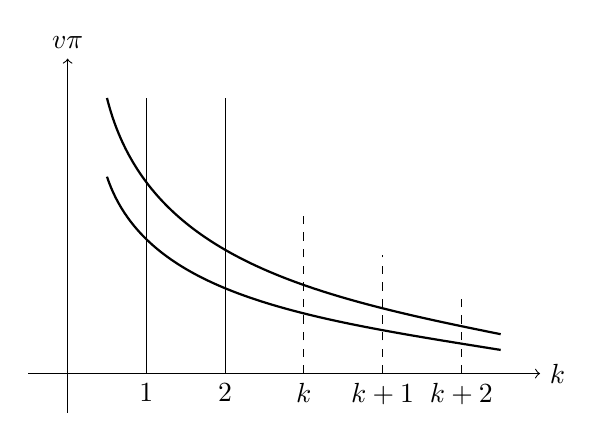
\begin{tikzpicture}
\draw[->] (-0.5,0) -- (6,0) node[right] {$k$};
\draw[->] (0,-0.5) -- (0,4) node[above] {$v\pi$};
\draw (1,0) -- (1,3.5);
\draw (2,0) -- (2,3.5);
\node at (1,0) [below] {$1$};
\node at (2,0) [below] {$2$};
\node at (3,0) [below] {$k$};
\node at (4,0) [below] {$k+1$};
\node at (5,0) [below] {$k+2$};
\draw[dashed] (3,0) -- (3,2);
\draw[dashed] (4,0) -- (4,1.5);
\draw[dashed] (5,0) -- (5,1);
\draw[thick] (0.5,3.5) .. controls (1,1.5) and (3,1) .. (5.5,0.5);
\draw[thick] (0.5,2.5) .. controls (1,1) and (3,0.7) .. (5.5,0.3);
\end{tikzpicture}
\end{center}

\end{document}
